
\chapter{Line Integrals}

This chapter covers the following ideas. 

% A list of objectives for the chapter
%\begin{enumerate}
%\item ...
%\end{enumerate}

\begin{enumerate}
\item Describe how to integrate a function along a curve. Use line
  integrals to find the area of a sheet of metal with height
  $z=f(x,y)$ above a curve $\vec r(t)=\langle x(t),y(t)\rangle$ and the average
  value of a function along a curve.
\item Find the following geometric properties of a curve: centroid,
  mass, center of mass, moments of mass, moments of inertia, and radii
  of gyration.
\end{enumerate}

%%% Local Variables: 
%%% mode: latex
%%% TeX-master: "../multivariable-calculus"
%%% End: 
%$

\section{Line Integrals}

The integral $\int_a^b f(x)dx$ is an integral in the plane of a function
$y=f(x)$ over the interval $(a,b)$.  This integral gives the area of
the region above the interval (assuming $f\geq 0$).  The interval $(a,b)$
can be parametrized as the curve $C\colon\vec r(t)= \langle x,0\rangle, a\leq x\leq
b$, and arc length can be computed using $\int_C ds = \int_a^b |\vec
r'(x)|dx = \int_a^b 1 dx = b-a$. Notice that $ds=dx$ on the interval. A
little piece of area $dA$ is width $ds$ times height $f$, so area can
be computed using the integral $\int_C dA = \int_C f ds = \int_a^b f(x)|\vec
r^\prime(x)|dx = \int_a^b f(x) dx$. 

To find the area of a metal sheet that has height $z=f(x,y) $ over a
curve $ \vec r(t)=\langle x(t),y(t)\rangle $, we approximate the area by breaking
the curve up into little pieces $\Delta s$. The length of each piece is
approximated by {$ \Delta s \approx \sqrt{\Delta x^2 +\Delta y^2} =|\vec r\vp(t)|dt$}. The
height along a small portion of the sheet can be approximated by
$f(\vec r(t))$. A small piece of area $\Delta A$ is approximately $f\Delta s
$. To find the total area, we sum the approximate areas $A\approx \sum f\Delta s$.
Taking a limit as $\Delta s$ approaches zero gives the integral $ \int_C f \,ds
= \int_a^b f |r'(t)|dt,$ (recall that $ds = |r'| dt = \text{ speed } \times
d(\text{time})$).  This integral is called a line integral.  To
calculate a line integral, parametrize a curve $C$ and then compute
the integral using the formula $ \int_C f\,ds = \int_a^b f |r'(t)|dt $. This
formula extends first-semester calculus integration along an interval
to all dimensions.  Line integrals are used to find work done by a
non-constant force to move an object along an arbitrary path. Work
leads to the concepts of flow, circulation, and flux, and is central
in understanding how energy is used to generate power.

\begin{example}
\marginpartop{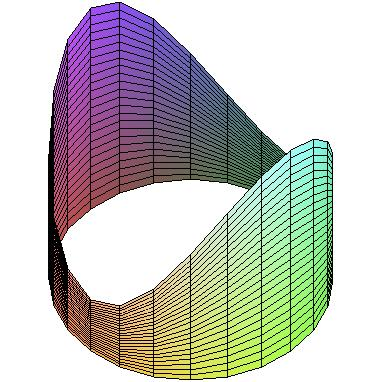
\includegraphics[width=\marginparwidth]{06-LineIntegrals/support/sheet-2}}%
 To find the area of a sheet of metal above the unit circle with
  height given by $f=x^2+4y^2$, first parametrize the curve $C\colon \vec
  r(t) = \langle\cos t,\sin t\rangle$, $0\leq t\leq 2\pi$. Then compute $A = \int_C f\,ds =
  \int_0^{2\pi} ((\cos t)^2 + 4 (\sin t)^2) \,|\langle-\sin t,\cos t\rangle|\,dt =
  \int_0^{2\pi} (\cos^2 t + 4 \sin^2 t) (1)\,dt$. To solve this integral,
  we can use integration tables, technology, or the trig identities
  $\cos^2 t= \frac{1+\cos 2t}{2}$ and $\sin^2 t = \frac{1-\cos
    2t}{2}$. This gives $$\int_0^{2\pi} \frac{1+\cos 2t}{2} +4 \frac{1-\cos
    2t}{2}dt = \int_0^{2\pi} \frac{5}{2} - \frac{3\cos 2t}{2}dt =
  \left.\left(\frac{5}{2}t - \frac{3\sin 2t}{4}\right)\right|_0^{2\pi} = 5\pi.$$
\end{example}

\begin{example}
\marginpartop{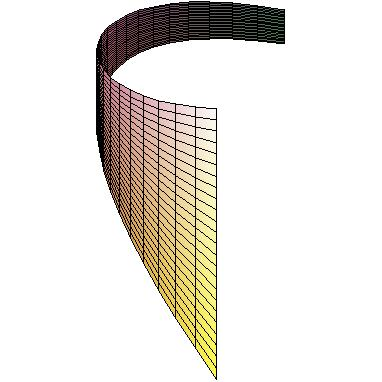
\includegraphics[width=\marginparwidth]{06-LineIntegrals/support/sheet-1}}%
The area of a sheet of metal above the curve $\vec
r(t)=\langle t,t^2\rangle$ for $-1<t<2$, with height given by
{$f=(x+2)(y+2)$}, is 
$\int_{-1}^{2}(t+2)(t^2+2)\sqrt{(1)^2+(2t)^2}\,dt 
= \int_{-1}^{2} (t+2)(t^2+2)\sqrt{1+4t^2}\,dt$. Solving this integral is
rather time consuming, and technology will quickly get an answer.
\end{example}

Please spend some time sharpening your integration skills (in
particular $u$ substitution and integration by parts), but do not
spend so much time doing complex integrals that you do not get to
practice the new ideas.


\section{Physical Applications}
We now develop average value, centroid, mass, center of mass, moment
of inertia, and radius of gyration. There are examples at the end of
this section of how to do all of this, as well as a ``Short Version''
which summarizes the ideas found herein. I strongly suggest you read
all of this at least once. It is okay if it doesn't all make sense
before discussion in class.  Reading it will help you understand, as
well as help you learn to read more complex mathematical ideas. 

\subsection{Average Value - how do you average infinitely many things}

The average of a finite number of values is $y_1,\ldots,y_n$ is
$\frac{1}{n}\sum_{i=1}^n y_i$. To extend this to an infinite average
value, we use ``weighted averages.'' If a value $y$ occurs more than
once in a list of numbers to be averaged, let $y_1,\ldots,y_n$ be the
distinct values to be averaged and $c_i$ be the number of times $y_i$
occurred. The total number of values to be averaged is $C=\sum_{i=1}^n
c_i$ and the average of these values is $\frac{1}{C}\sum_{i=1}^n c_iy_i =
\sum_{i=1}^n \frac{c_i}{C}y_i = \sum_{i=1}^n w_i y_i$. The number
$w_i=\frac{c_i}{C}$ is called a weight corresponding to $y_i$, and it
represents the proportion of times $y_i$ occurs in the total number of
values. 

\begin{example}
 The average of $1,1,3,4,4,4,4$ can be computed by
  considering the three distinct values $y_1=1, y_2=3, y_3=4$ which
  occur with frequency $c_1=2, c_2=1, c_3=4$. The number of values is
  $C=c_1+c_2+c_3=7$ and the weights are
  $w_1=\frac{2}{7},w_2=\frac{1}{7},w_3=\frac{4}{7}$.  The average of
  these values is $\sum_{i=1}^3 w_i y_i =
  \frac{2}{7}(1)+\frac{1}{7}(3)+\frac{4}{7}(4) = 3$.

\end{example}

Much more could be
said about weighted averages and their importance in mathematics and
practical applications. The sum of the weights $w_i$ is always 1
because each weight represents a portion of the total, and adding up
all these portions gives 100\% of the total.

\subsubsection{Average value by using weighted averages}
The average value of a function is an extension of finite averages to
an infinite average of the output values of the function. Consider a
function $f(x,y,z)$ which represents the temperature at any point
$(x,y,z)$ in space. If a particle travels along the space curve given
by $C\colon\vec r (t)=\langle x,y,z\rangle$ for $a\leq t\leq b$, the average value
of $f$ along this space curve will be an average of the infinitely
many temperature values along $C$. Divide $C$ into tiny portions (by
dividing the interval $(a,b)$ up into many pieces
$a=t_0<t_1<t_2<\cdots<t_{n-1}<t_n=b$) and pick a representative point 
 $\vec r(t_k)$ for each portion of the curve. Assuming the heat
$f$ is continuous, the heat 
$f_{i}=f(\vec r(t_i))$ at this representative point 
is approximately the same as the heat $f$ for every point $\vec r(t)$
on the curve for $t_{k-1}\leq t\leq t_{k}$. If each portion of the curve has
length $\Delta s_i$, then the proportion of the total length located in the
$i$th bit of curve is $\frac{\Delta s_{i}}{s}$, where $s$ is the arc length
of $C$. We use this proportion as our weight in a weighted average
because it gives the proportion of times a heat $f$ value would occur
even in an infinite setting. The weighted average of $f_{i}$ using the
weights $w_{i}=\frac{\Delta s_{i}}{s}$ is approximately the average value
of $f$, 
$AV\approx \sum_{i=1}^n \frac{\Delta s_{i}}{s}f(\vec r(t_i)) 
= \frac{1}{s} \sum_{i=1}^n f(\vec r(t_i)) \Delta s_{i}$. As $\Delta s_{i}$
approaches zero, we obtain the integral formula $AV=\frac{1}{s}\int_C
f(\vec r(t))\,ds$. Often people will just write $AV=\frac{1}{s}\int_C f
\,ds$, where it is implied that you replace $x,y,z$ with what they are
in terms of $t$.  Remember that $ds = |\vec r\vp(t)|dt$. 

\subsubsection{Average Value by finding a constant that can be used to
replace $f$}
If we multiply both sides of the formula $AV=\frac{1}{s}\int_C f \,ds$ by
arc length $s$, then we obtain the formula $(AV)(s) = \int_C f \,ds$, or
$(AV)\int_C 1 \,ds = \int_C f \,ds$. Since $AV$ is a constant, bring it inside
the integral giving $\int_C (AV) \,ds = \int_C f \,ds$.  The last formula has a
geometric interpretation: average value ($AV$) is a constant value
such that if you replaced the integrand $f(x,y,z)$ with $AV$, then you
would obtain the same line integral. The formula used in previous calculus classes is
$AV (b-a) =\int_a^b f(x)dx$. The area underneath $f$ from $a$ to $b$ is
given by $\int_a^b f(x)dx$. Average value is the height $AV$ of a
rectangle with the same width which has the same area as the area
under $f$.  If you were to take an ant farm where the top of the sand
was given by the function and shake it so that the sand all leveled
off, then the height of the sand when you were done shaking would be
the average value.  

\bigskip

We have purposefully discussed average value in two different ways:
(1) using weighted averages, (2) replacing $f$ with $AV$ in the
formula $\int_C (AV) \,ds = \int_C f \,ds$ and solving for $AV$ which gives
$AV=\frac{1}{s}\int_C f \,ds$.  These two ideas will be used in the
applications which follow. 

\subsection{Centroid}
The centroid $(\bar x,\bar y,\bar z)$ of an object is the point in
space whose {$x,y,z$}-values are the average {$x,y,z$}-values.  The
average value formula gives $\bar x = \frac{1}{s}\int_C x\,ds, \bar y =
\frac{1}{s}\int_C y\,ds, \bar z = \frac{1}{s}\int_C z\,ds$, which when written
in vector form is equivalent to $ \langle\bar x,\bar y,\bar z\rangle =
\frac{1}{s}\int_C  \langle x,y,z\rangle \,ds$. In terms of weighted averages,
the weight attached to each point is $\frac{ds}{s}$, the proportion of
arc length corresponding to each point.

\subsection{Density and Mass}

A density is the measure of a quantity per unit something. The
derivative $\frac{dy}{dx}$ is a measure of change in $y$ per unit
change in $x$. A change $dy$ of a function for some given change $dx$
is computed by multiplying the density $\frac{dy}{dx}$ by the change
$dx$, giving us the familiar equation $dy = \frac{dy}{dx}dx$. Adding
up these approximate changes in $y$ gives the integral formula $\int_a^b
dy = \int_a^b f' dx$ which measures the total change in $y$ from $a$ to
$b$ (or more commonly called the fundamental theorem of calculus). 
Hopefully this was a review. The new idea is that density is the
measure of a quantity per unit something.

Mass density $\delta(x,y,z)$ in space is a measure of mass per unit volume,
i.e $\text{density}=\frac{\text{mass}}{\text{unit volume}}$. The
(mass) density of water is found by calculating the mass of some
quantity of water and dividing by its volume. The metric unit system
was created so that 1 kg of water occupies 1 liter of space, giving a
density of 1kg/L (this is how we connect mass and volume). Different
substances have different densities.  If you mix oil and water, the
density of oil is less than water which is why the oil and water
separate themselves with the oil on top and the water underneath.
When an object is made out of many different materials, the density of
the object may differ depending on where in the object you are.  This
is why we write $\delta(x,y,z)$, to reinforce the idea that density may
vary based upon which portion of the object you are considering.  To
find the mass of an object with constant density, we just multiply the
density by its volume.

If we consider an object that is located in space along a space curve
$C\colon\vec r (t)=\langle x,y,z\rangle$ for $a\leq t\leq b$, then it is more
convenient to think of density as mass per unit arc length.  This
gives us a density $\delta(x,y,z)$ at each point on the curve, and then the
mass of each little portion of the curve can then be approximated by
multiplying the density of one point of the piece by the length of
each little piece.

The density  (mass per unit length) at a point is the mass that would
result if points with the same density were to occupy 1 unit of arc
length. If points of density $\delta(x,y,z)$ occupied a curve of length $\Delta
s$, then the mass of that curve would be $\Delta m = \delta(x,y,z)\Delta s$. (Do you
see an integral formula coming? If so, try to write it down before you
read any more.) If we know the density of an object $\delta(x,y,z)$ for 
all $(x,y,z)$ along a curve $C\colon\vec r(t)$, then divide the curve $C$
into little arcs $\Delta s_{i}$. Approximate the mass of each arc by
assuming the density is constant on each little piece, which gives $\Delta
m_{i} \approx \delta(x_i,y_i,z_i)\Delta s_{i}$. Total mass is found by adding up these
little bits of mass, and then taking a limit as $\Delta s_{i}\to 0$, which
gives $m=\int_C \delta \,ds$.  In differential notation, we write $dm = \delta ds$,
 so $m=\int_C dm$ (mass is found by adding up little bits of mass).  

\subsection{Center of Mass and First Moments}

The center of mass of an object is the weighted average of the
$(x,y,z)$ values where the weights are given by the proportion of mass
$\frac{dm}{m}$ corresponding to each region. The integral formula is
$\langle\bar x,\bar y,\bar z\rangle = \frac{1}{m}\int_C
\langle x,y,z\rangle dm = \frac{1}{m}\int_C \langle x,y,z\rangle dm$. The
difference between center of mass and centroid is that for a centroid,
we assume $\delta$ is constant, so it comes out of the integral and cancels to give $\frac 1 s \int_C \langle x,y,z\rangle\,ds$.  

\subsubsection{First Moments of mass}
The quantities $M_{yz}=\int_C x dm, M_{xz}=\int_C y dm$, and  $M_{xy}=\int_C z
dm$ which appear in the formula for center of mass are called the
first moments of mass about the $yz$ plane, about the $xz$ plane, and
about the $xy$ plane, respectively. These first moments of mass are a
weighted directed measure of distance from a plane. 
To find the first moment about the plane $x=c$, we note that the
distance to the plane $x=c$ is $x-c$, so the moment is $M_{x=c}=\int_C
(x-c)dm$.  The center of mass is the value $\bar x$ such that the
moment about the plane $x=\bar x$ is zero, or $\int_C(x-\bar x)dm = 0$.
Since $\bar x$ is a constant, this becomes $0=\int_C x dm - \bar x \int_C dm$
or $\bar x m = \int x dm=M_{yz}=M_{x=0}$. Hence center of mass can be
written in terms of moments by the formulas
$\bar x =M_{yz}/m,\bar y =M_{xz}/m, \bar z = M_{xy}/m$. 
There are various applications of moments in statistics, physics, and
mathematics, however the language used in each field is slightly
different. Wikipedia has a wealth of information about this topic.

\subsection{Inertia}

Kinetic energy of a moving object is $\displaystyle KE=\frac{1}{2}
mv^2$, where $m$ is the mass and $v$ is the velocity. Imagine a
particle moving in a circular path of radius $r$ about some axis.  Let
$\theta(t)$ be the angle the particle is at at time $t$.  The net distance
the particle travels between times $t_1$ and $t_2$ is
$r\theta(t_2)-r\theta(t_1)$, so $r\theta(t)$ is the position function of the
particle.  The velocity is {$ v=\frac{d}{dt}(r\theta)=r\frac{d\theta}{dt} =
  r\omega(t) $}, where we call $\omega(t)$ the rotational velocity at time
$t$. The kinetic energy of a rotating particle is thus {$\displaystyle
  KE=\frac{1}{2} m(r\omega)^2 = \frac{1}{2} m r^2\omega^2$}. Since an object
which is rotating has particles at different radii, finding the total
kinetic energy of a rotating object requires more work.  We divide the
object into little pieces with mass {$\Delta m$} and rotate each little
piece around the axis of rotation, giving {$\displaystyle \Delta KE=
  \frac{1}{2} \Delta m r^2 \omega^2$}.  Summing gives us {$\displaystyle KE \approx \sum
  \frac{1}{2} \Delta m r^2 \omega^2 = \frac{1}{2} \omega^2 \sum r^2 \Delta m$}. Taking a
limit gives {$\displaystyle KE = \frac{1}{2} \omega^2 \int r^2 dm$}, where
{$r$} is the radius of rotation of a small piece of mass $dm$.  The
quantity {$I=\int r^2 dm$} is called a moment of inertia about an axis of
rotation (or a second moment). We can then write kinetic energy as
$KE=\frac{1}{2}v^2 m = \frac{1}{2}\omega^2 I$. Notice that a moment of
inertia takes the place of mass in rotational kinetic energy.

In 3D, the radius of rotation about an axis is the distance to the
axis.  The radius of rotation about the $x$-axis is $\sqrt{y^2+z^2}$,
the radius of rotation about the $y$-axis is $\sqrt{x^2+z^2}$, and the
radius of rotation about the $z$-axis is $\sqrt{x^2+y^2}$ (just leave
off $x$ when finding distance to $x$ axis, leave off $y$ when finding
distance to $y$-axis, and leave off $z$ when finding distance to $z$
axis). This gives the formulas for the moments of inertia for a curve
$C$ with density $\delta$ to be $I_x = \int_C (y^2+z^2)\delta \,ds$, $I_y = \int_C
(x^2+z^2)\delta \,ds$, and $I_z = \int_C (x^2+y^2)\delta \,ds$ (we squared each
distance, hence the square roots disappear).  The single formula $I=\int
r^2 dm$ describes all of these formulas. You can find the moment of
inertia about any line. All you have to do is find a formula for the
distance from a point on the curve to the axis of rotation.

\subsubsection{Radii of Gyration}

The radius of gyration $R$ about an axis is a positive radius $R$ such
that if we replace $r^2$ with $R^2$ in the moment of inertia equation,
we would have $\int R^2 dm = \int r^2 dm$. This means $R^2 m = I$ or
$R=\sqrt{I/m}$. The radius of gyration about the $x$-axis is $R_x =
\sqrt{I_x/m}$, and similarly $R_y = \sqrt{I_y/m}$ and $R_z=
\sqrt{I_z/m}$. The radius of gyration about an axis is a rotational
center of mass. It is used in studying energy, and is often used to
simplify complex problems. This derivation was similar to us finding
the center of mass, where we replaced $x$ with $\bar x$ to obtain the
equality $\int \bar x dm = \int x dm$ or $\bar x =(\int x dm)/m$.

\subsection{Summary}
Most everything we learned above is summarized below in differential
notation.  Essentially, in this learning module, you are learning to
use and derive differential formulas to find quantities such as area,
centroids, mass, center of mass, moments, moments of
inertia, and radii of gyration.  Let $C\colon r(t)$ be a curve.
\begin{itemize}
\item Area: $dA = fdx$ for an interval, $dA=fds $ for a curve.
\item Average Value: $(AV) s = \int f \,ds$, so $AV=\frac 1 s \int f\,ds$.
\item Centroid: $\langle\bar x,\bar y,\bar z\rangle s =\int
\langle x,y,z\rangle\, ds$, so $\langle\bar x,\bar y,\bar z\rangle= \frac 1 s \int \langle x,y,z\rangle\,ds$ (find average $x,y,z$ values)
\item Mass: $dm = \delta ds $, where $\delta$ is a function giving the density at a point.
\item Center of Mass: Just replace $s$ with $m$ in centroid,
$\langle\bar x,\bar y,\bar z\rangle m = \int_C \langle x,y,z\rangle dm$,
where $M_{yz}=\int_C \bar x dm = \int x dm$ is a first moment of mass, so $\bar x = M_{yz}/m$.  Similarly for $M_{xz}$ and $M_{xy}$.
\item $I = \int r^2 dm$ is a moment of inertia, and $\int R^2 dm = \int r^2 dm$
gives $R^2 m =I$ or $R=\sqrt{I/m}$ as the radius of gyration (where
$r$ represents the generic distance from a point in space to the axis
of rotation).
\end{itemize}
I strongly suggest that you start each problem from a differential
formula, and then work from there to convert it to a line integral in
terms of t that you can evaluate.  This practice will make parts of
the next two units much easier.


\subsection{Examples}
Here is an example of each idea with a single curve. When you create
your lesson plan, I suggest that you focus on one particular space
curve, density, and function.  Then show how all the formulas are
developed from there.

Consider the elliptical helix $C\colon\vec r (t) = \langle3\sin t, 4\cos t,
t\rangle$ for $0\leq t\leq 2\pi$.  The arc length differential is $$ds = |\vec
r'(t)|dt = \sqrt{(3\cos t)^2 + (-4\sin t)^2+1^2}dt = \sqrt{9\cos^2
t+16\sin^2 t+1}dt.$$ Arc length is then  $$s=\int_C ds =
\int_{0}^{2\pi}\sqrt{9\cos^2 t+16\sin^2 t+1}dt.$$

The centroid of this curve is found using the integral formulas (which
are too ugly to bother solving by hand):
\begin{align*}
\bar x &= \frac{\int_C x ds}{\int_C ds} = \frac{\int_{0}^{2\pi}(3\sin
t)\sqrt{9\cos^2 t+16\sin^2 t+1}\,dt}{\int_{0}^{2\pi}\sqrt{9\cos^2 t+16\sin^2
t+1}\,dt}\\
\bar y &= \frac{\int_C y ds}{\int_C ds} = \frac{\int_{0}^{2\pi}(4\cos
t)\sqrt{9\cos^2 t+16\sin^2 t+1}\,dt}{\int_{0}^{2\pi}\sqrt{9\cos^2 t+16\sin^2
t+1}\,dt}\\
\bar z &= \frac{\int_C z ds}{\int_C ds} = \frac{\int_{0}^{2\pi}(t)\sqrt{9\cos^2
t+16\sin^2 t+1}\,dt}{\int_{0}^{2\pi}\sqrt{9\cos^2 t+16\sin^2 t+1}\,dt}
\end{align*}
or you can use the single vector formula (which means compute the
three integrals above) 
$$\langle\bar x,\bar y,\bar z\rangle = \frac{\int_C \langle x,y,z\rangle
ds}{\int_C ds} = \frac{\int_{0}^{2\pi} \langle3\sin t, 4\cos t,
t\rangle\sqrt{9\cos^2 t+16\sin^2 t+1}\,dt}{\int_{0}^{2\pi}\sqrt{9\cos^2
t+16\sin^2 t+1}\,dt}$$

If the curve represents a wire in space with density given by $\delta
(x,y,z) = x^2+y^2z$ kg/L, then $dm = \delta ds$, and we can calculate the
centroid as follows (just replace $ds$ in the above formulas with
$dm=\delta ds$):
\begin{align*}
m=&\int dm = \int_C \delta ds = \int_{0}^{2\pi}((3\sin t)^2+(4\cos
t)^2(t))\sqrt{9\cos^2 t+16\sin^2 t+1}\,dt\\
\bar x &= \frac{\int x dm}{\int dm}= \frac{\int_C x \delta ds}{\int_C \delta ds} =
\frac{\int_{0}^{2\pi}(3\sin t)((3\sin t)^2+(4\cos t)^2(t))\sqrt{9\cos^2
t+16\sin^2 t+1}\,dt}{\int_{0}^{2\pi}((3\sin t)^2+(4\cos t)^2(t))\sqrt{9\cos^2
t+16\sin^2 t+1}\,dt}\\
\bar y &= \frac{\int y dm}{\int dm}= \frac{\int_C y \delta ds}{\int_C \delta ds} =
\frac{\int_{0}^{2\pi}(4\cos t)((3\sin t)^2+(4\cos t)^2(t))\sqrt{9\cos^2
t+16\sin^2 t+1}\,dt}{\int_{0}^{2\pi}((3\sin t)^2+(4\cos t)^2(t))\sqrt{9\cos^2
t+16\sin^2 t+1}\,dt}\\
\bar z &= \frac{\int z dm}{\int dm}= \frac{\int_C z \delta ds}{\int_C \delta ds} =
\frac{\int_{0}^{2\pi}(t)((3\sin t)^2+(4\cos t)^2(t))\sqrt{9\cos^2
t+16\sin^2 t+1}\,dt}{\int_{0}^{2\pi}((3\sin t)^2+(4\cos t)^2(t))\sqrt{9\cos^2
t+16\sin^2 t+1}\,dt}
\end{align*}
The first moments of mass, second moments of inertia, and radii of
gyration are given by:
\begin{align*}
M_{yz} &= \int x dm = \int_C x \delta ds = \int_{0}^{2\pi}(3\sin t)((3\sin t)^2+(4\cos
t)^2(t))\sqrt{9\cos^2 t+16\sin^2 t+1}\,dt\\
M_{xz} &= \int y dm = \int_C y \delta ds = \int_{0}^{2\pi}(4\cos t)((3\sin t)^2+(4\cos
t)^2(t))\sqrt{9\cos^2 t+16\sin^2 t+1}\,dt\\
M_{xy} &= \int z dm = \int_C z \delta ds = \int_{0}^{2\pi}(t)((3\sin t)^2+(4\cos
t)^2(t))\sqrt{9\cos^2 t+16\sin^2 t+1}\,dt\\
I_x &= \int r^2 dm =\int y^2+z^2 dm =\int_{0}^{2\pi}[(4\cos t)^2+(t)^2]((3\sin
t)^2+(4\cos t)^2(t))\sqrt{9\cos^2 t+16\sin^2 t+1}\,dt\\
I_y &= \int r^2 dm =\int x^2+z^2 dm =\int_{0}^{2\pi}[(3\sin t)^2+(t)^2]((3\sin
t)^2+(4\cos t)^2(t))\sqrt{9\cos^2 t+16\sin^2 t+1}\,dt\\
I_z &= \int r^2 dm =\int x^2+y^2 dm =\int_{0}^{2\pi}[(3\sin t)^2+(4\cos
t)^2]((3\sin t)^2+(4\cos t)^2(t))\sqrt{9\cos^2 t+16\sin^2 t+1}\,dt\\
&R_x=\sqrt{I_x/m},\
R_y=\sqrt{I_y/m},\
R_z=\sqrt{I_z/m},\
\end{align*}





%%% Local Variables: 
%%% mode: latex
%%% TeX-master: "../multivariable-calculus"
%%% End: 





